
In this section we illustrate our methodology on simulated data.
The parameters of our model we must choose in order to simulate data are the value of $\beta$,
the $(f,h)$ pair of functions, and the error distribution.
We must also choose distributions to draw $x$ and $z$ from and the sample size.
We will always use $\beta=1$.


%#nonlinear strong
%fnls = function(x,z) {return(x[1] + .5*x[1]*x[2] + .5*x[2]^2 + z[1] + z[2]*x[1]+ .5*z[2]^2)}
%hnls = function(x) {return(x[1] - .25*x[1]*x[2]^3 + x[3])}
%#linear strong
%fls = function(x,z) {return(x[1] + x[2] + x[3] + z[1] + z[2])}
%hls = function(x) {return((x[1] - x[2] + .5*x[4]))}

We will consider a nonlinear pair of $(f,h)$:

\begin{eqnarray}\label{eq:sim-nonlinfuns}
f(x,z) & = & x_1 + .5 \, x_1 x_2 + .5 x_2^2 + z_1 + z_2 x_1 + .5 z_2^2  \label{eq:sim-nonlinfuns-f} \\
h(x) & = & x_1 - .25 x_1 x_2^3 + x_3 \label{eq:sim-nonlinfuns-h}
\end{eqnarray}

and a linear pair of $(f,h)$:

\begin{eqnarray}\label{eq:sim-linfuns}
f(x,z) & = & x_1 + x_2 + x_3 + z_1 + z_2 \label{eq:sim-linfuns-f}\\
h(x) & = & x_1 - x_2 + .5 x_4\ . \label{eq:sim-linfuns-h}
\end{eqnarray}

The nonlinear functions are chosen to be simple polynomials.
This is not too different from what a practitioner might try but 
a practitioner may have difficulty finding the exact right polynomial terms in practice.
The linear functions are chose to be a simple as possible while having $h$ not too similar to the $x$ part of $f$.

For the error distribution we use:
\begin{eqnarray}\label{eq:sim-error}
\epsilon_T & = & \sigma_T \, Z_T \\
\epsilon_Y & = & \gamma Z_T + \sigma_Y Z_Y
\end{eqnarray}
where $(Z_T,Z_Y)$ are indepenent $t_\nu$ random variables with $\nu=5$.
We let $\sigma_T = 1$ and $(\gamma,\sigma_Y) = (\frac{1}{\sqrt{2}},\frac{1}{\sqrt{2}})$. 
Note that a linear combination of independent $t$ random variables is not a $t$ random variable so that the error $\epsilon_Y$ has
a non-standard distribution.
Clearly $\gamma$ controls the degree of dependence between $\epsilon_T$ and $\epsilon_Y$.
With these choices, both errors have the same variance as the $Z$'s and the correlation is $1/\sqrt{2} \approx .707$.
The pair of errors $(\epsilon_{Ti},\epsilon_{Yi})$ are iid over observations.

Each coordinate of both $x$ and $z$ are iid uniform on the interval $(-2,2)$.
For $x$, we simulate $x_j, j=1,2,\ldots,10$ and for $z$ we simulated $z_j, j=1,2, \ldots 5$.
So, there are 10 $x$ variables and 5 potential $z$ instruments.
Notice that in the nonlinear case (Equations  \ref{eq:sim-nonlinfuns-f} and \ref{eq:sim-nonlinfuns-h}),
$f$ uses only $(x_1,x_2,z_1,z_2)$ while $h$ uses only $(x_1,x_2,x_3)$.
The method is given all 10 $x$ and all 5 $z$ and the two BART models in IVBART have to learn which variables matter.
In the linear case (Equations \ref{eq:sim-linfuns-f} and \ref{eq:sim-linfuns-h}),
$f$ and $h$ use $(x_1,x_2,x_3,z_1,z_2)$ and $(x_1,x_2,x_4)$ respectively.

We consider four different simulation scenarios by letting the sample
size $n$ be 2,000 or 500 and letting the functions be nonlinear or
linear.  We draw 90 samples and run MCMC estimation of each of the
three models IVBART, linear-normal, and linear-DPM on each of the 90
samples.

All IVBART results are obtained using a default prior specification
explained in Section~\ref{subsec:sim-prisens} and, in more detail, in
Section~\ref{details}.  Results for the linear-normal and linear-DPM
models are obtained using the default prior specifications provided by
the functions \texttt{rivGibbs} and \texttt{rivDP} in the \texttt{R}
package \texttt{bayesm} \citep{RPbayesm}.

\subsection{Inference for $\beta$}\label{subsec:sim-beta-inf}

Figure~\ref{fig:alldraws} displays the MCMC draws of $\beta$ from the three models
IVBART, linear-normal, and linear-DPM.
The four plots in the figure correspond to our four simulation scenarios.

The top-left plot of Figure~\ref{fig:alldraws}  corresponds to the scenario where we have simulated 2,000 observations (90 times) using
the nonlinear specifications of $f$ and $h$.
From each simulated data set we obtain a set of MCMC draws of $\beta$ and we combine all the draws into one large
set of draws and then use a density estimate to represent the draws.
The point of the paper is clearly illustrated by the  fact that the distribution of draws
from the IVBART model (solid density curve) is much tigher around the true value of $\beta=1$ than
the densities for the linear-normal model (dashed) or the linear-DPM model (dot-dash).
By figuring out the functions $f$ and $h$ from the data, with no user input, IVBART is able to get
a more precise inference for $\beta$ than is obtained by simply assuming the functions are linear.

From the top-right plot in Figure~\ref{fig:alldraws} we see that with $n=2,000$ and linear functions,
the inference from the IVBART model is very similar to that obtained from the two linear models linear-normal and 
linear-DPM.
The IVBART model is slightly more upward biased.

The two bottom plots of Figure~\ref{fig:alldraws} show that when the sample size is smaller, as we expect, 
things are tougher for the flexible model.
IVBART still produces draws closer to $\beta$ in the nonlinear case but there is some downward bias.
In the linear case, the IVBART draws are again slightly upwardly biased but still quite similar to the linear methods.

Table~\ref{tab:rmse} summarizes the results by reporting the root mean squared error (RMSE) of
the $\beta$ draws, again averaged over all MCMC draws and all simulations.
We also report the relative RMSE for each simulation scenario by dividing the RMSE of each model
by the minimum over the three models.
With $n = 2,000$ and nonlinear functions, IVBART has the smallest RMSE and the RMSE for the linear-normal model
is 86\% larger while the RMSE for the linear-DPM model is 77\% larger.
With $n = 500$, and nonlinear functions, IVBART is again the best with the linear-normal and linear-DPM
models being 42\% and 35\% worse.
In the linear cases, the linear models win, but the IVBART model is at most 28\% worse.
The numbers in Table~\ref{tab:rmse} reinforce the message of Figure~\ref{fig:alldraws}.
When there is strong nonlinearity, IVBART is much better and not too much worse in the linear case.

\begin{figure}
\hspace*{-.3in}
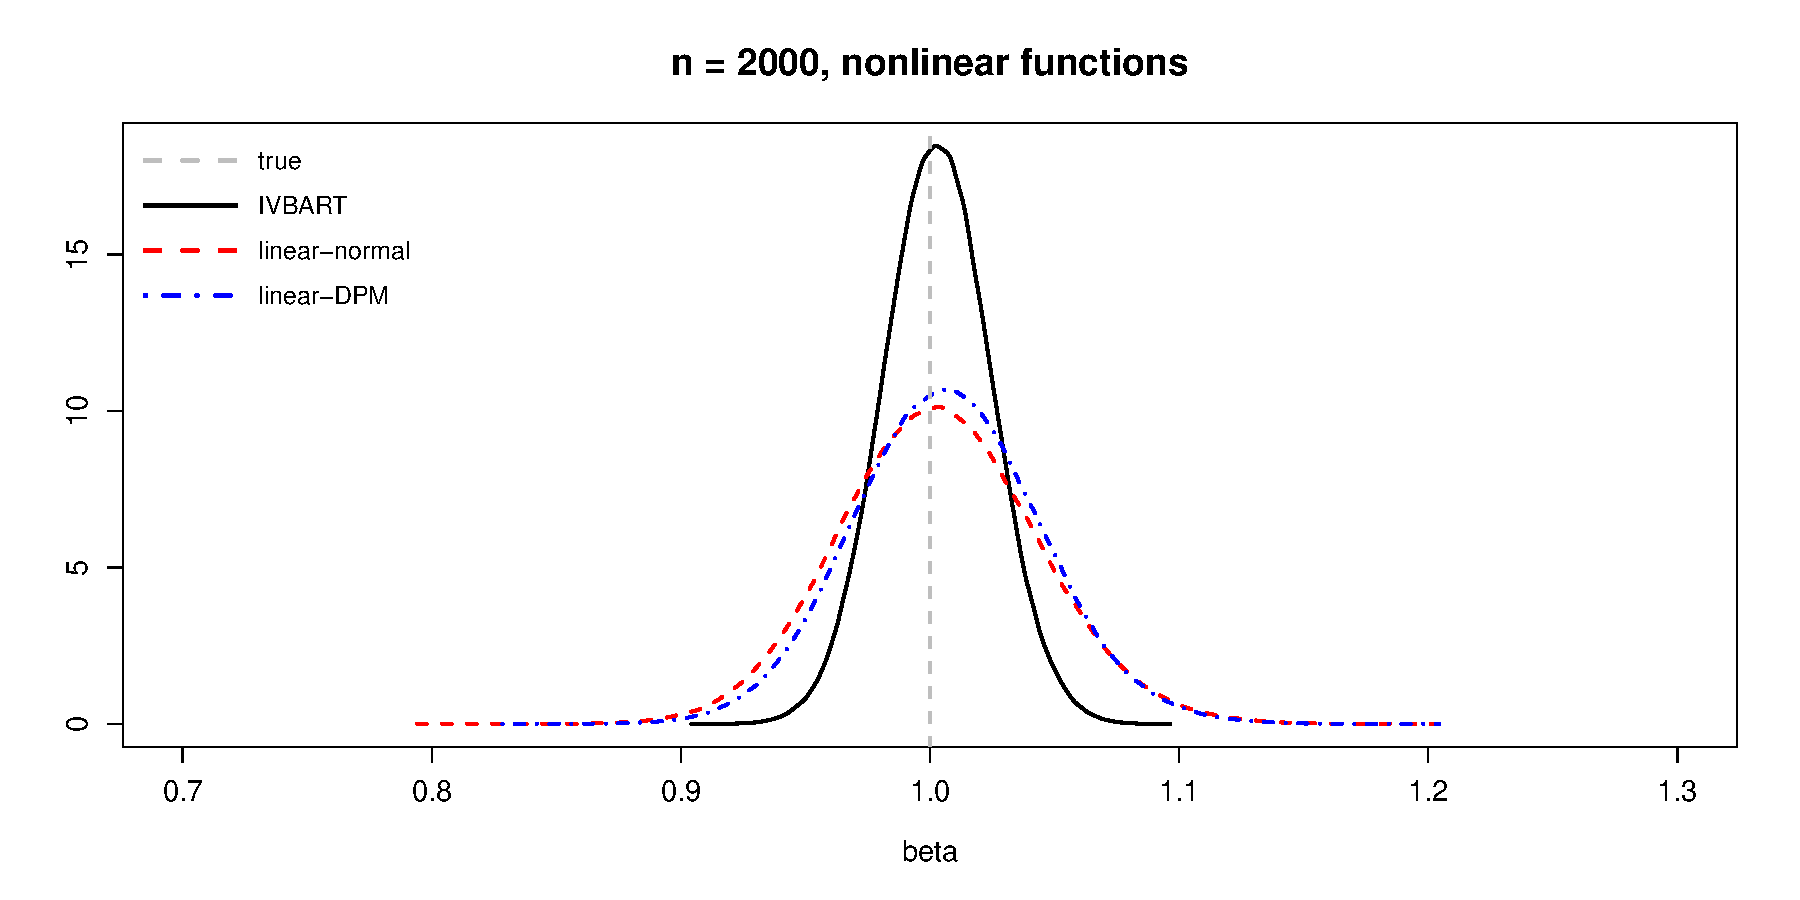
\includegraphics[scale=.3]{14-11_1-2_2000_alldraws_densities.pdf}
\hspace{.1in}
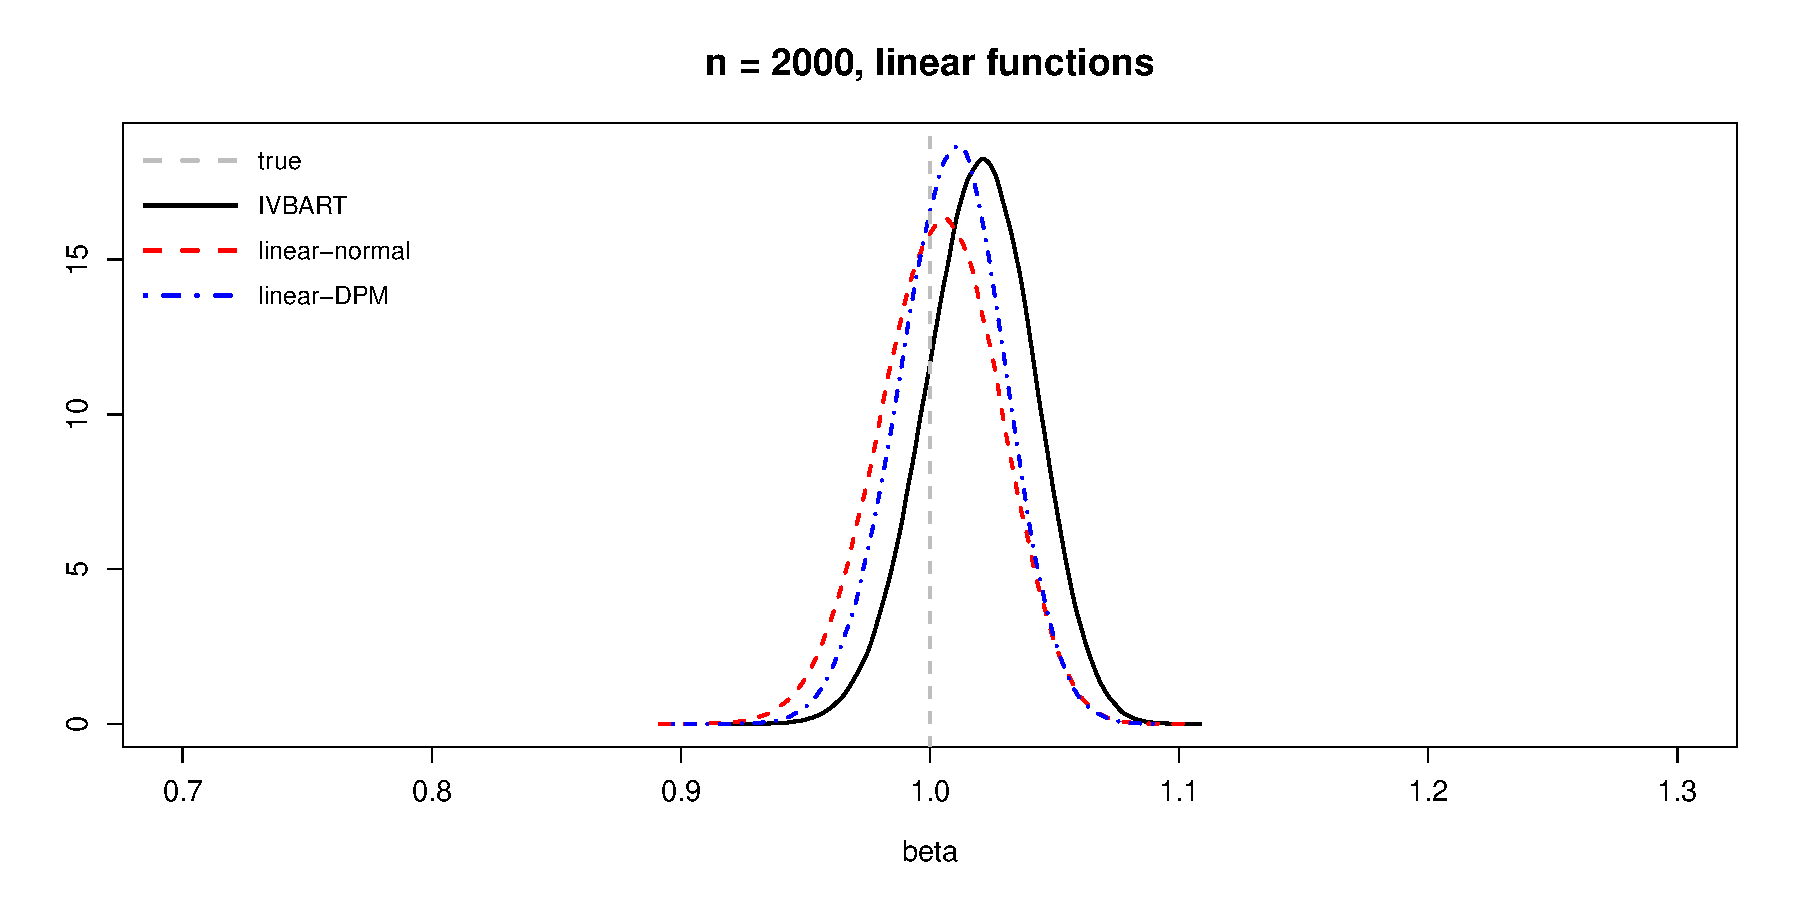
\includegraphics[scale=.3]{14-31_1-2_2000_alldraws_densities.pdf} \\
\hspace*{-.3in}
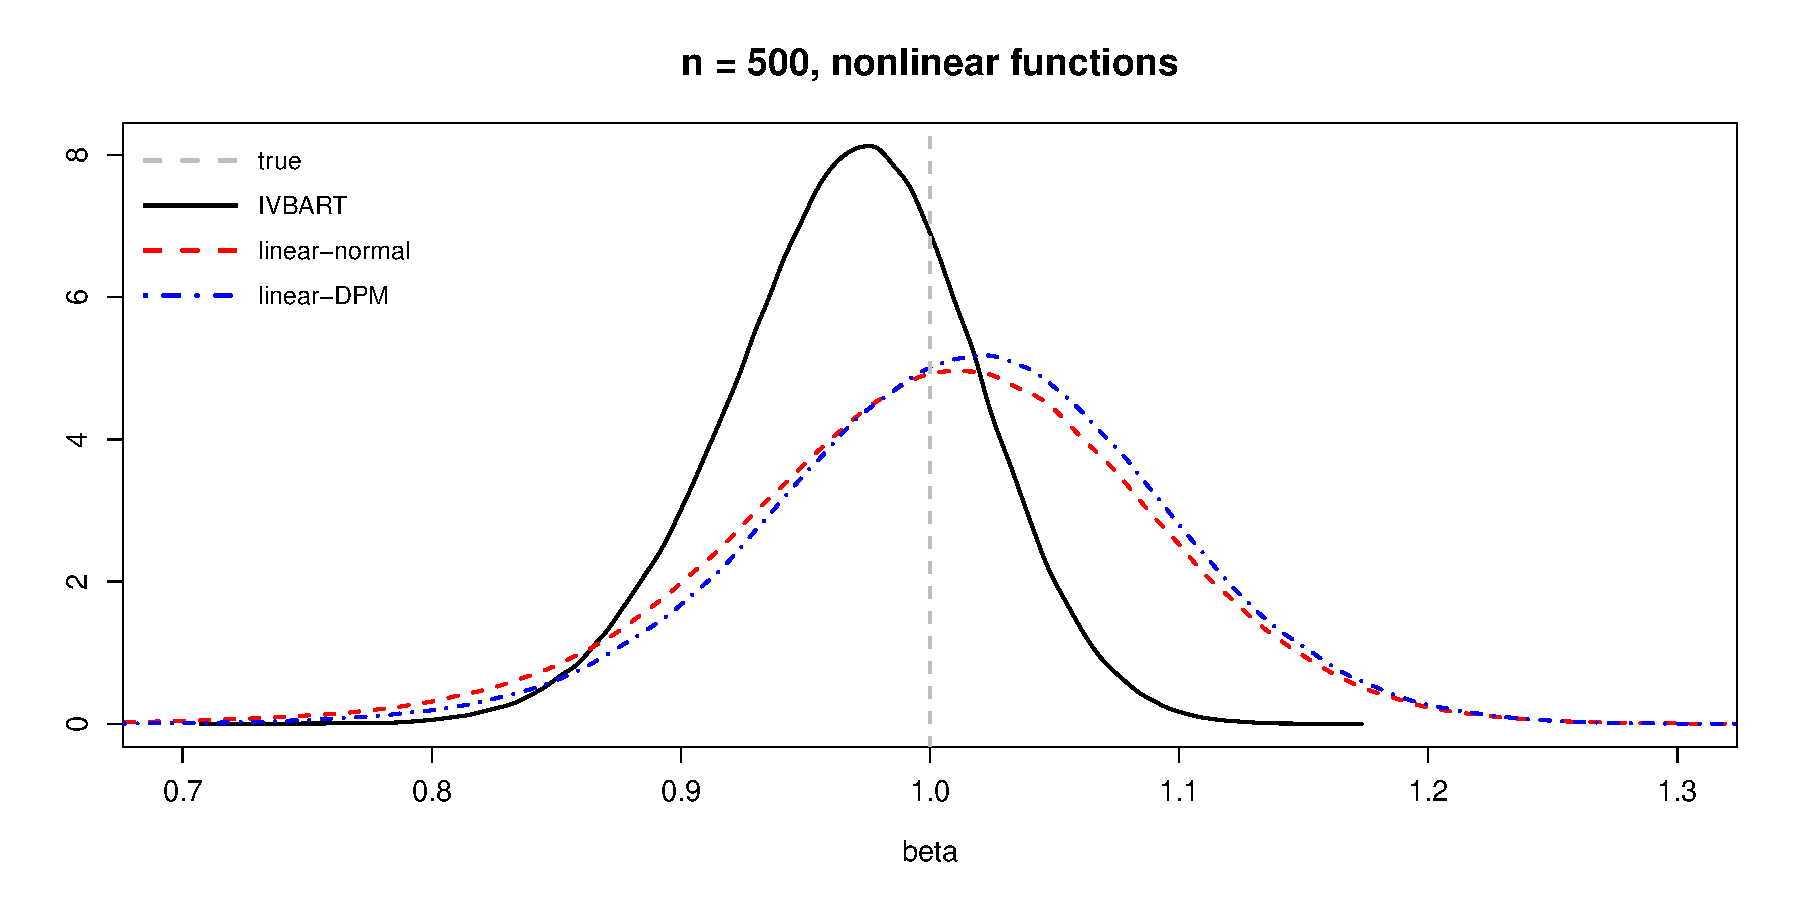
\includegraphics[scale=.3]{14-11_1-2_500_alldraws_densities.pdf}
\hspace{.1in}
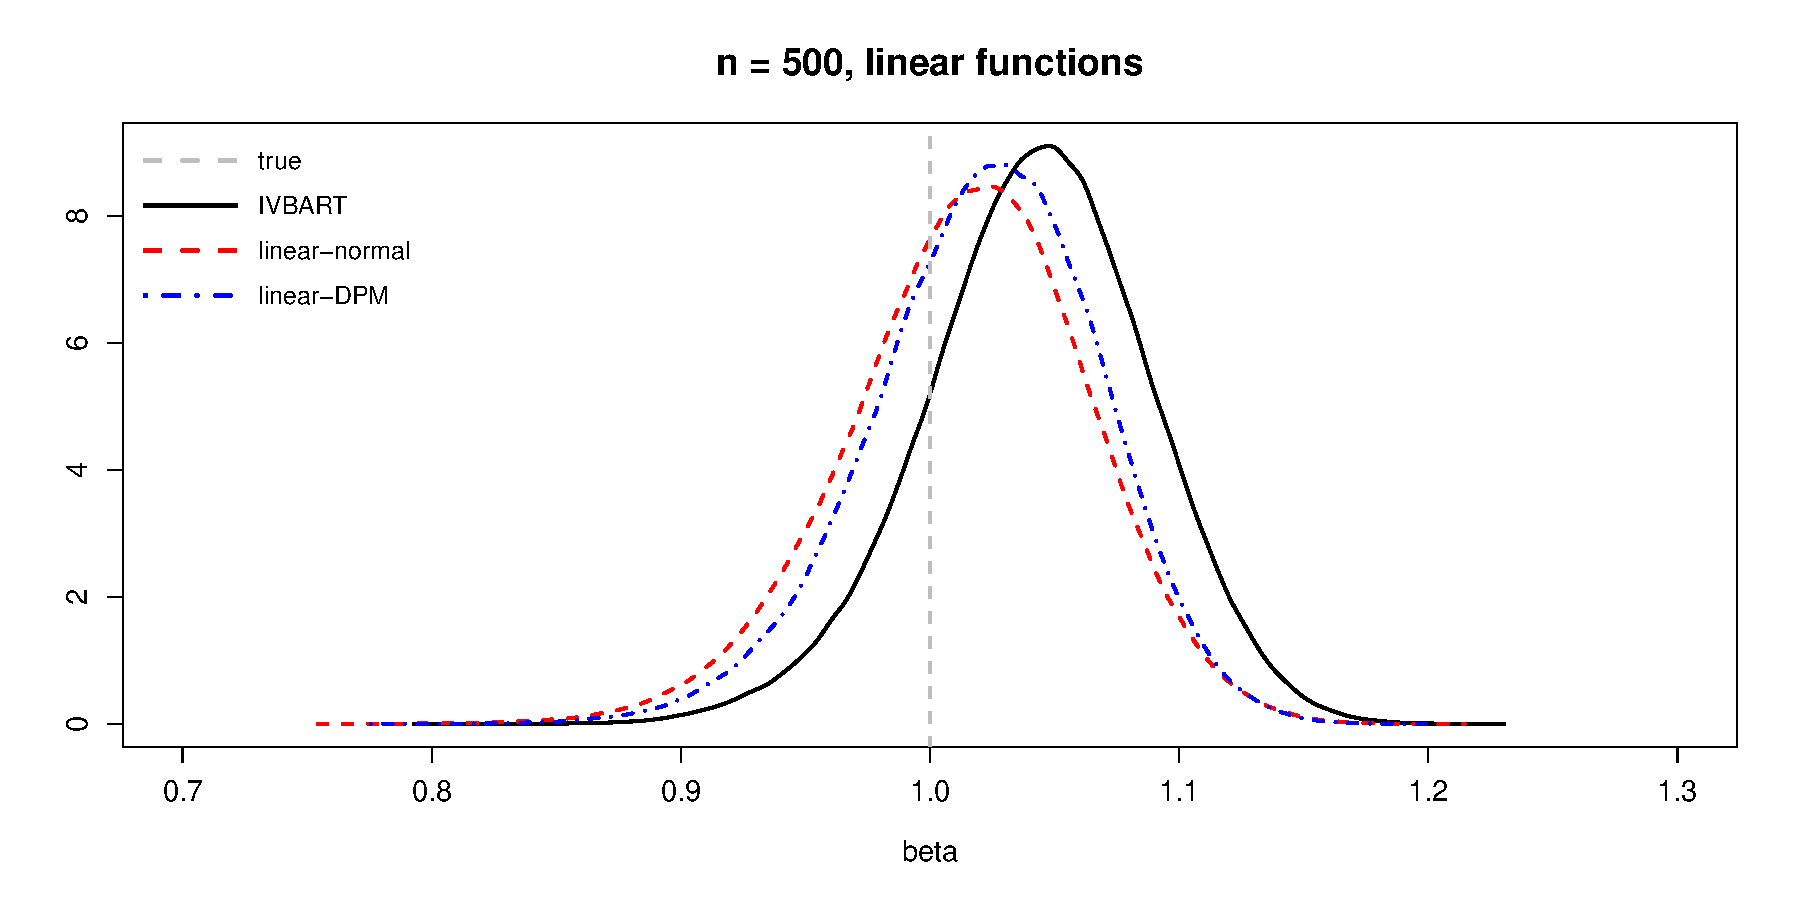
\includegraphics[scale=.3]{14-31_1-2_500_alldraws_densities.pdf} 
\caption{%
Densities estimates from MCMC draws of $\beta$ using the IVBART (solid), the linear-normal (dashed) and linear-DPM (dot-dash) models.
Each density estimate is based on all MCMC draws from all 90 data simulations.
In the top two figures, $n=2,000$.
In the bottom two figures, $n=500$.
In the left two figures, the data sets were simulated using the nonlinear function.
In the right two figures, the data sets were simulated using the linear functions.
\label{fig:alldraws}}
\end{figure}

\begin{table}[tbp]  \centering
\begin{tabular}{l|rrr}
 & IVBART & linear-normal & linear-DPM \\
\hline
n=2,000, nonlinear & (0.022, 1.000) & (0.040, 1.858) & (0.038, 1.769) \\
n=2000, linear & (0.029, 1.275) & (0.024, 1.059) & (0.023, 1.000) \\
n=500, nonlinear & (0.060, 1.000) & (0.085, 1.417) & (0.080, 1.348) \\
n=500, linear & (0.062, 1.220) & (0.051, 1.000) & (0.051, 1.002)
\end{tabular}
\caption{%
RMSE and relative RMSE. 
Rows are for our four simulation scenarios and columns are for our three models.
Each table entry reports (RMSE, relative RMSE).
The relative RMSE for each simulation scenario is obtained by dividing the RMSE
for each of the three models by the minimum over the three models. 
\label{tab:rmse}
}
\end{table}

Figure~\ref{fig:sim-ints} displays 95\% posterior intervals for each simulation and each model.
The four plots again correspond to our four simulation scenarios.
Within each plot, each short vertical line segment represents a 95\% interval obtained from the 
.025 and .975 quantiles of the MCMC $\beta$ draws.
The first 90 line segments display the posterior intervals for the IVBART method while the 
second and thirds sets of 90 display the intervals for the linear-normal and linear-DPM models.
In each plot the final three (thicker) vertical line-seqments display the .025 and .975 quantiles for all draws
combined for each method (as in Figure~\ref{fig:alldraws} and Table~\ref{tab:rmse}).
In the top plot we clearly see the good performance of the IVBART model as the intervals are shorter
and located near the true value of $\beta$.
In the linear cases (second and fourth plot) we see that IVBART is not too different from the linear
models but somewhat biased upward.
In the nonlinear case with $n = 500$, the IVBART intervals are smaller than the linear ones but slightly
downard biased.
We discuss the bias further in Section~\ref{subsec:sim-prisens}.

\begin{figure}
\centerline{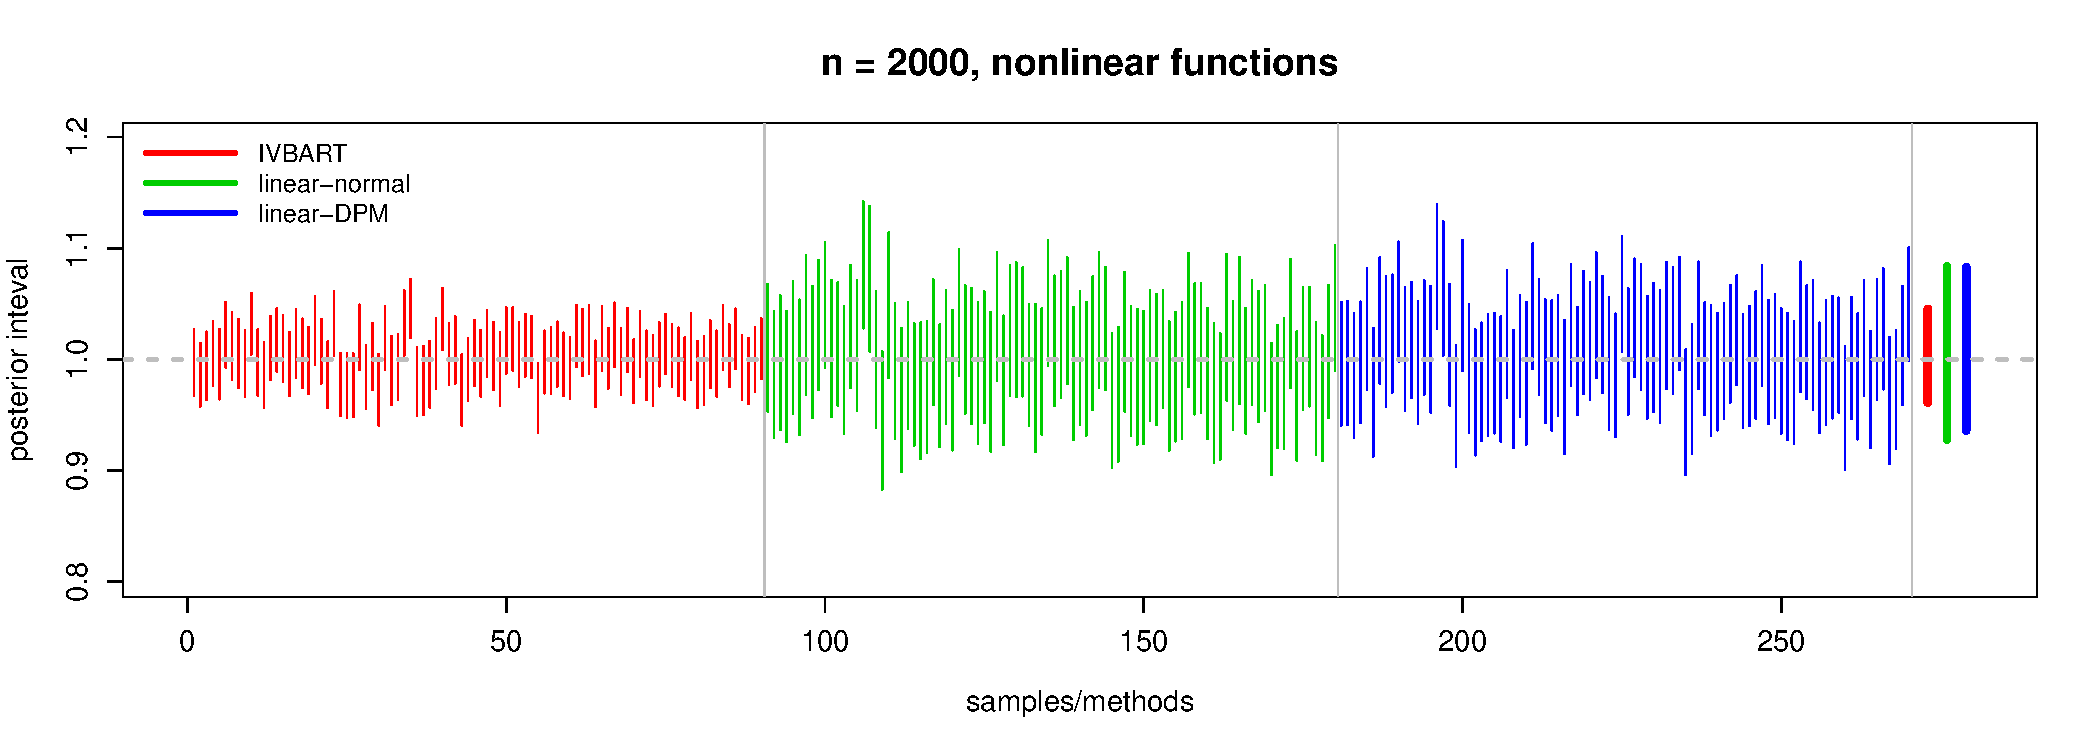
\includegraphics[scale=.35]{14-11_1-2_2000_intervals.pdf}} 
\centerline{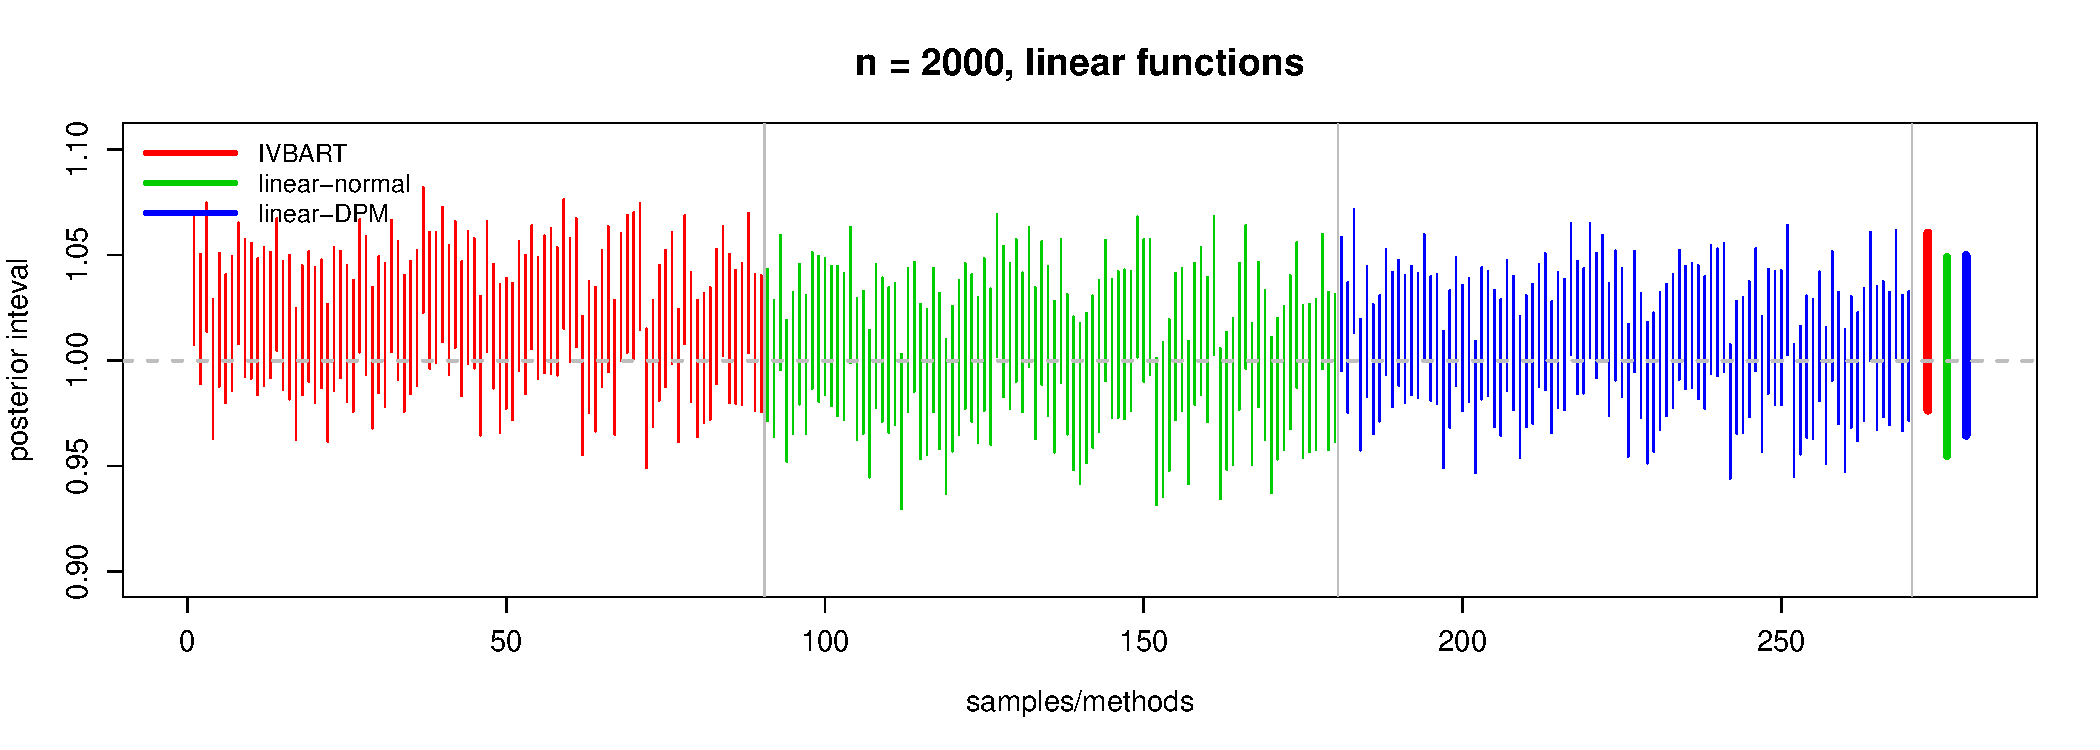
\includegraphics[scale=.35]{14-31_1-2_2000_intervals.pdf}} 
\centerline{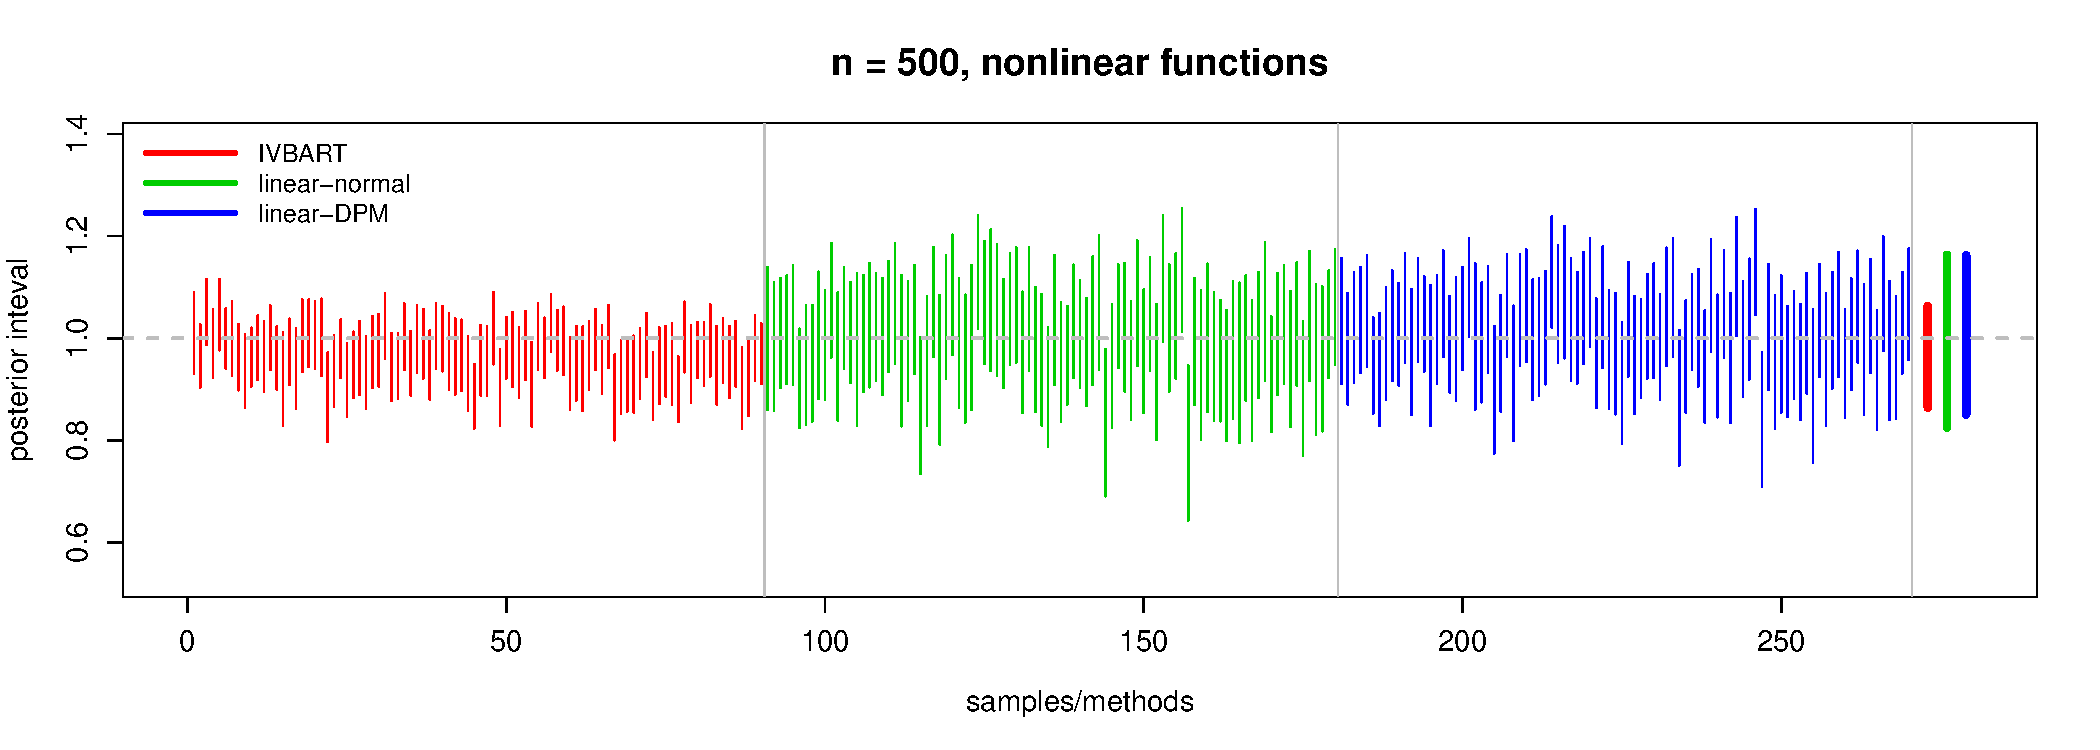
\includegraphics[scale=.35]{14-11_1-2_500_intervals.pdf}}  
\centerline{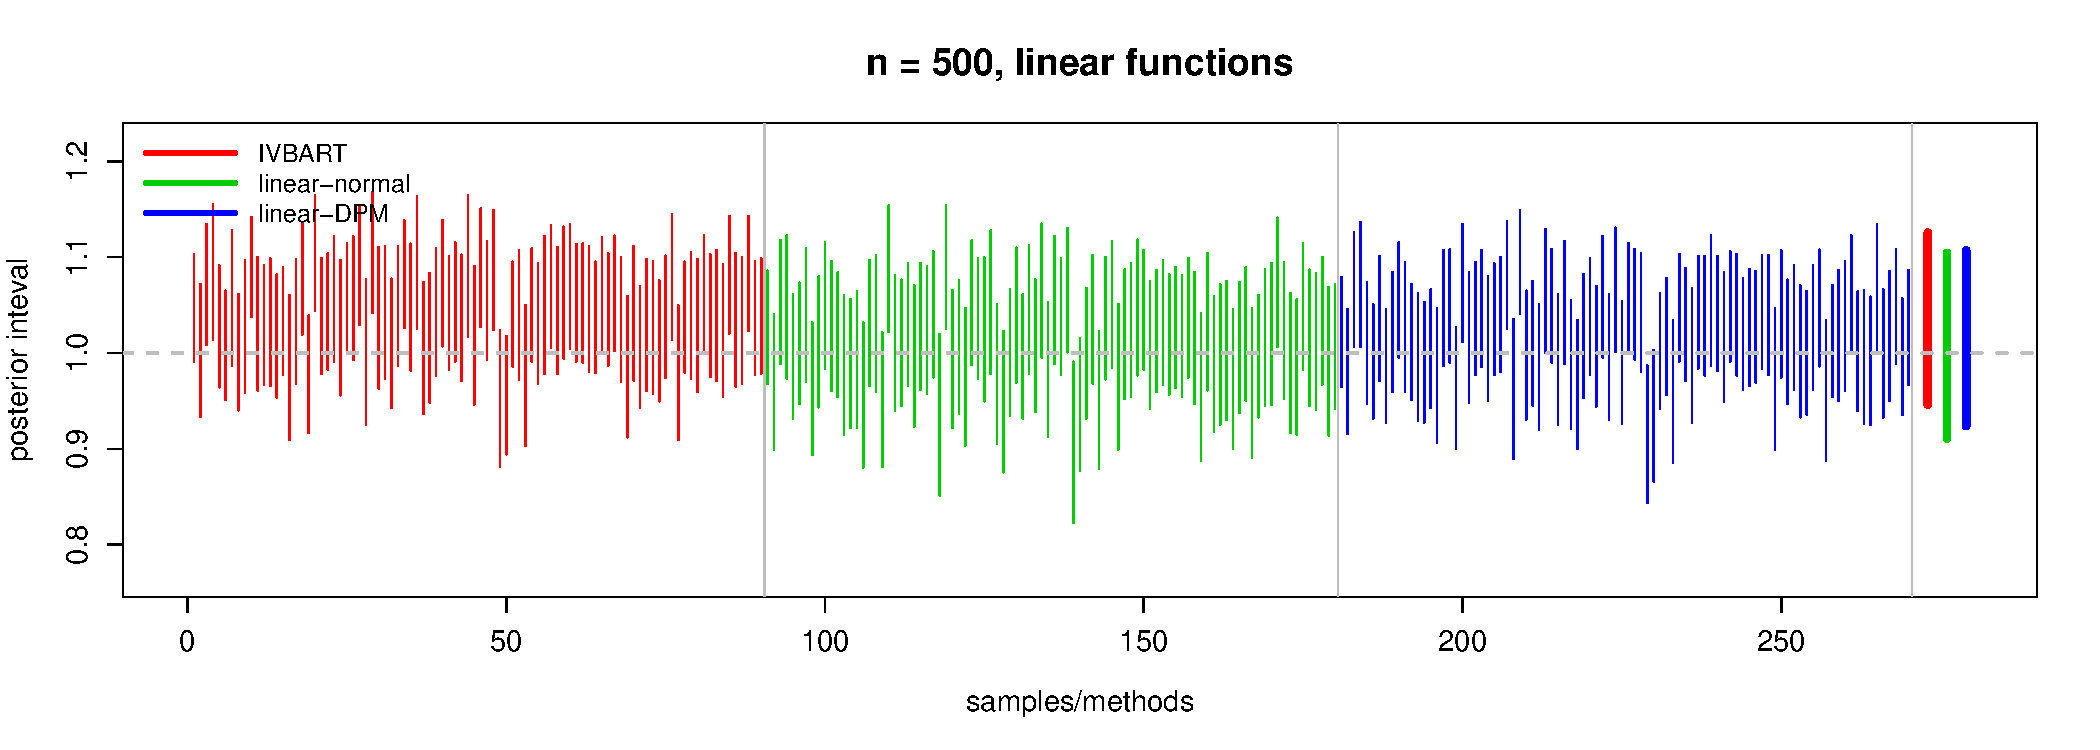
\includegraphics[scale=.35]{14-31_1-2_500_intervals.pdf}}
\caption{%
95\% Posterior intervals for $\beta$.
Each vertical segment represents a 95\% posterior interval.
Top two plots are for simlulation data sample size $n=2,000$ and the bottom two are for $n=500$.
Within each pair, the first is for the nonlinear functions and the second is for the linear functions.
Within each plot, the first 90 intervals are from IVBART while the second is from linear-normal and the third set of 90 is from linear-DPM.
The final three (thicker) intervals display .025 and.975 quantiles where all draw from all simulations are combined (as in Figure~\ref{fig:alldraws}).
\label{fig:sim-ints}}
\end{figure}

\subsection{Prior Sensitivity}\label{subsec:sim-prisens}

In the bottom-left plot if Figure~\ref{fig:alldraws} we see a bias in the inference for $\beta$.
We also see this in the third plot in Figure~\ref{fig:sim-ints}.
Two basic features of our model may be contributing to this bias.
First, even when $f$ and $h$ are linear, our model is intrinsically nonlinear in inferring $\beta$.
This is made clear in the Gibbs conditional for $\beta$ given in Section~\ref{betacond}.
Secondly, the extreme flexibility of our model makes our inference sensitive to the prior.
In Equations \ref{n-liniv1} and \ref{n-liniv2}, both the nonlinear functions ($f$ or $h$) and
the error terms ($\epsilon_T$ or $\epsilon_Y$) are capable of adaptively capturing the variation on
$T$ and $Y$.
Of course, the degree to which the variation in $T$ and $Y$ is captured by the functions as opposed to
the errors, will affect our inference for $\beta$.
When the data are sufficiently informative (top-left of Figure~\ref{fig:alldraws}) the prior is less
influential.  But for smaller sample sizes (bottom-left of Figure~\ref{fig:alldraws}) the prior may affect
our inference.

In \citep{ChipGeor10} great care is taken to develop a data dependent prior for the error term
and nonlinear function for the simple single equation predictive model.
In \citep{DPMBART}, the approach is extended to a single equation with nonparametric error estimation.
While we are working to extend these approaches to our IV model, we first take the alternative approach
of studying the prior sensitivity.
In our current model, emphasis is on the estimation of the causal parameter $\beta$
as opposed the predictive goal emphasized in \citep{ChipGeor10}.
In this case, we find the prior sensitivity approach helpful.
See also \citep{BCF} for  an important contribution to the problem of model and prior specification when
using BART type models for causal inference.

The key prior choices involve the BART priors for $f$ and $h$ and the priors for the DPM estimation
of the joint error distribution of $(\epsilon_T,\epsilon_Y)$.
Details for these prior choices are given in Section~\ref{details}.
In this section we give an overview of the prior choices and examine the sensitivity of our
inference to a key aspect of the prior.

The prior for the error term estimation follows \citep{CHMR08,ROSSI14}.
We first rescale both $T$ and $Y$ by subtracting off the sample mean and then
dividing by the sample standard deviation.  Draws of $\beta$ are then rescaled to return to the original units.
The error DPM prior is then designed to be informative, but flexible enough to cover the full range of the data.
Of course the scaling based on the sample mean and standard deviation is sensitive to the error distribution
but \citep{CHMR08} report good results for severly non-normal errors.
We also note that the results reported in Section~\ref{subsec:sim-beta-inf} provide further evidence
for the excellent performance of the \citep{CHMR08} approach.
Note that for a single equation, this is a much more spread out prior for the errors than used
in \citep{ChipGeor10} or \citep{DPMBART}.

For the priors on $f$ and $h$ we start with the very simple BART prior specification:
\begin{equation}
f(x,z) \sim N(0,\sigma^2_f), \;\; h(x) \sim N(0,\sigma^2_h),
\end{equation}
where $\sigma_f$ and $\sigma_h$ are prior parameters that must be chosen.
This remarkably simple prior specification is key the success of BART.
Given we have standardize both $T$ and $Y$ simple prior choices could be
$\sigma_f \approx 1.0$ and $\sigma_h \approx 1$.
The default used for all results in Section~\ref{subsec:sim-beta-inf} are 
$\sigma_f = 1.2$ and $\sigma_h = 1.2$.

While these choices are simple and motived by the data standardization, they
may be too spread out in that both the error and the functions are allowed to capture
all of the variation.  In \citep{ChipGeor10} and \citep{DPMBART} the priors on the error process
are tuned to guide the model towards exploring inferences where the error is smaller.
We now explore the sensitivity of our results to the choices of $\sigma_f$ and $\sigma_h$.

Figures \ref{fig:sim-prisens-500} and \ref{fig:sim-prisens-2000} present inference
for $\beta$ based on a single simulated data set.
Density estimates from MCMC draws of $\beta$ are presented where the prior choice is varied.
In Figure~\ref{fig:sim-prisens-500}, $n = 500$ while in Figure~\ref{fig:sim-prisens-2000}, $n = 2,000$.
In the top plot of each Figure, $\sigma_f$ and $\sigma_h$ are equal and varied in the set of values
$S_\sigma = \{.8,1,1.2,1.4\}$.
In the bottom plot of each figure all 16 possible combinations 
$\{(\sigma_f,\sigma_h): \sigma_f \in S_\sigma, \sigma_h \in S_\sigma \}$ are tried.
The thicker density  corresponds to the choice $(\sigma_f,\sigma_h) = (1.2, 1.2)$ used throughout
Section~\ref{subsec:sim-beta-inf}.

Clearly when is $n$ large (Figure~\ref{fig:sim-prisens-2000}) the results are fairly insensitive to the choice
of prior and indicative of a larger value for $\beta$ than suggested by the linear models.
When $n$ is smaller, (Figure~\ref{fig:sim-prisens-500}) the results are more sensitive to the prior, 
but we still have the correct suggestion that 
$\beta$ may be smaller than the values suggested by the linear models.


\begin{figure}
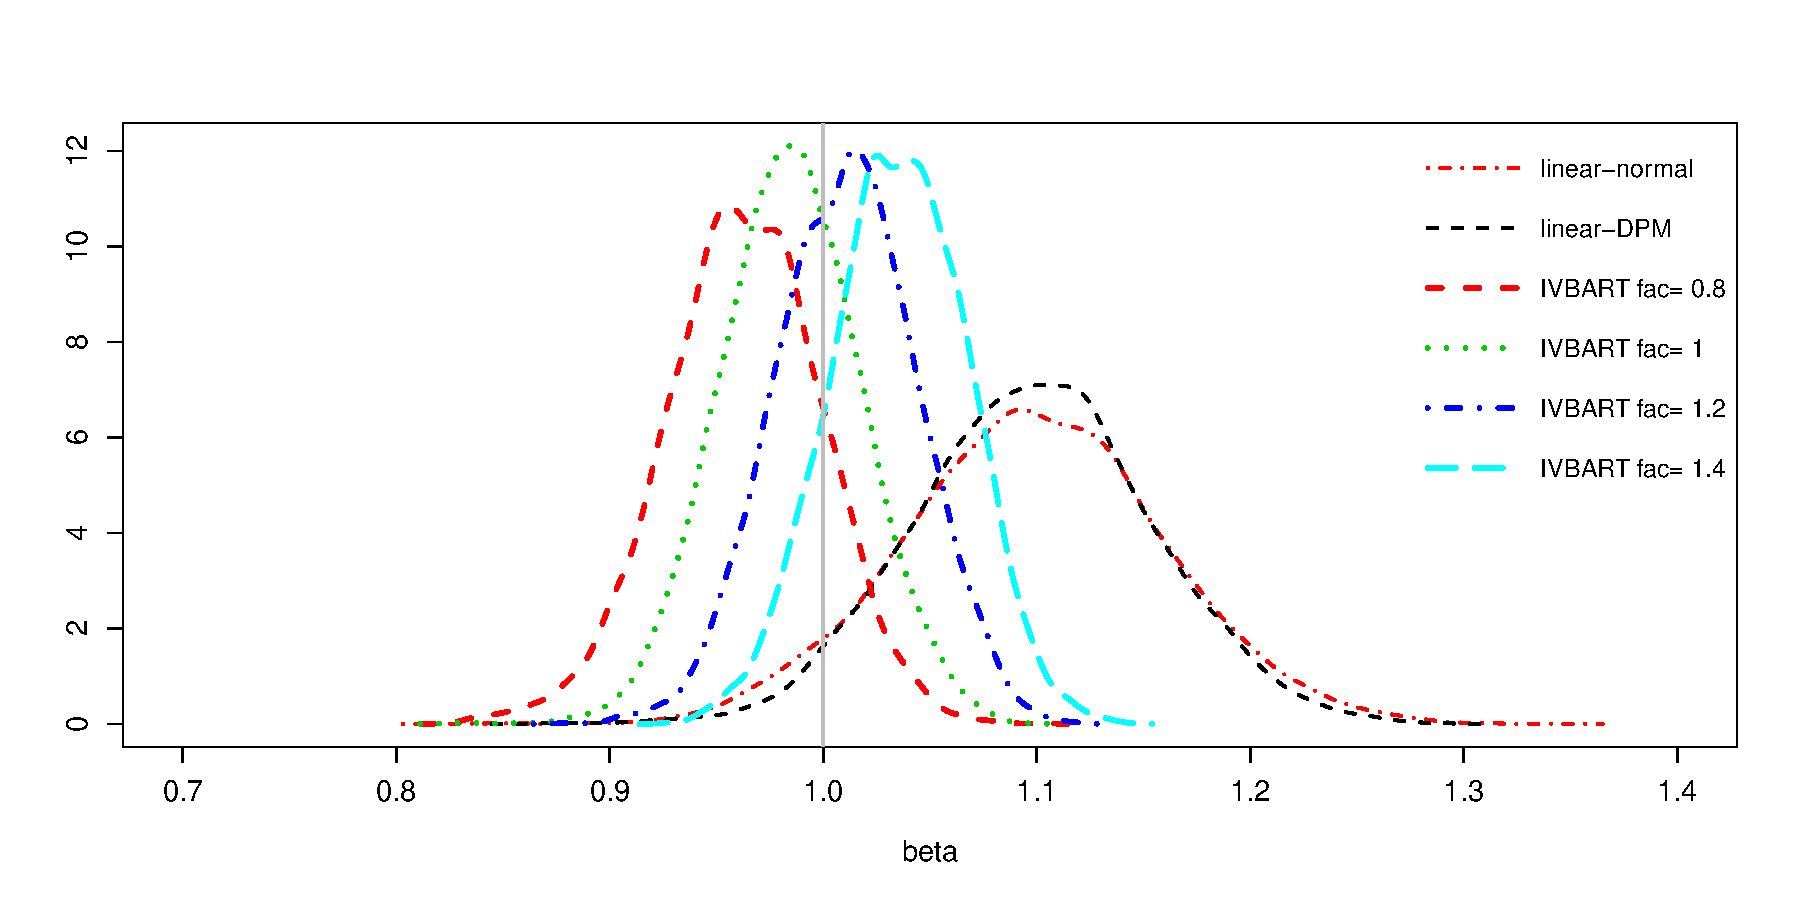
\includegraphics[scale=.6]{14-11_1-2_500_sim-prisens_1-way.pdf} \\
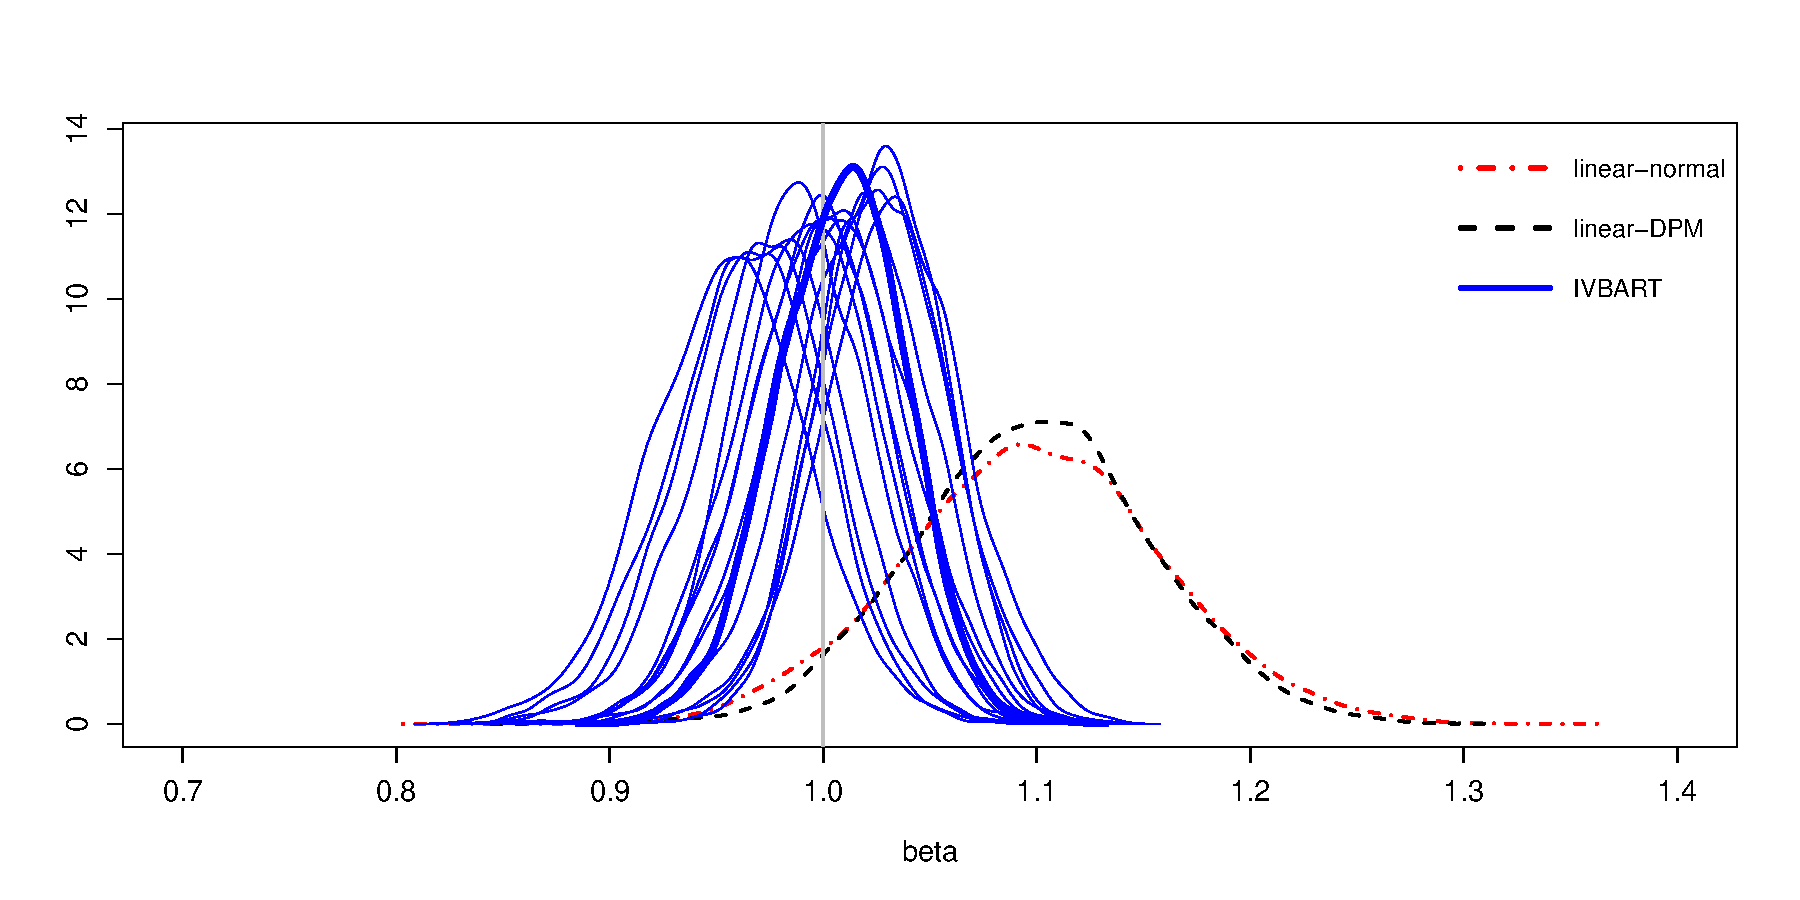
\includegraphics[scale=.6]{14-11_1-2_500_sim-prisens_2-way.pdf} 
\caption{%
Prior sensitivity with $n = 500$.
In the top plot $\sigma_f = \sigma_h$ and these values are varied in $S_\sigma = \{.8,1,1.2,1.4\}$.
In the bottom plot, all 16 density estimates obtained using $\sigma_f \in S_\sigma$ and $\sigma_h \in S_\sigma$
are shown.
The thicker density corresponds to $(\sigma_f,\sigma_h) = (1.2, 1.2)$.
Densities for draws from the linear-normal (dot-dash line) and linear-DPM (dashed line) models are also shown in each plot.
\label{fig:sim-prisens-500}}
\end{figure}

\begin{figure}
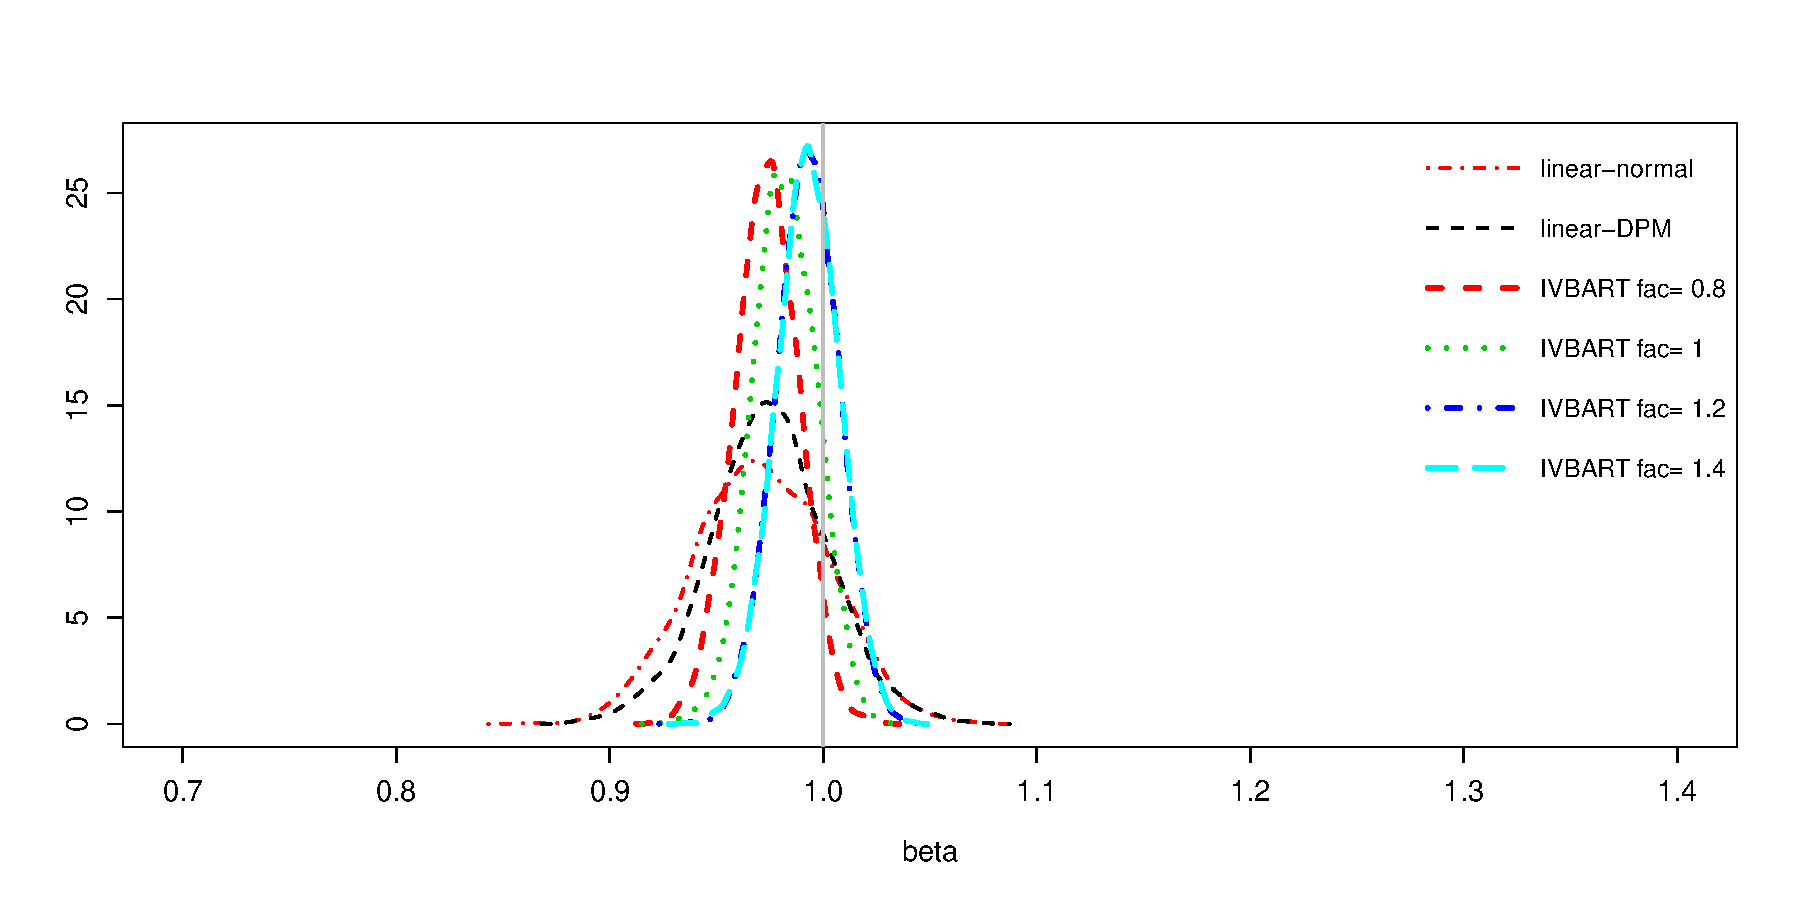
\includegraphics[scale=.6]{14-11_1-2_2000_sim-prisens_1-way.pdf} \\
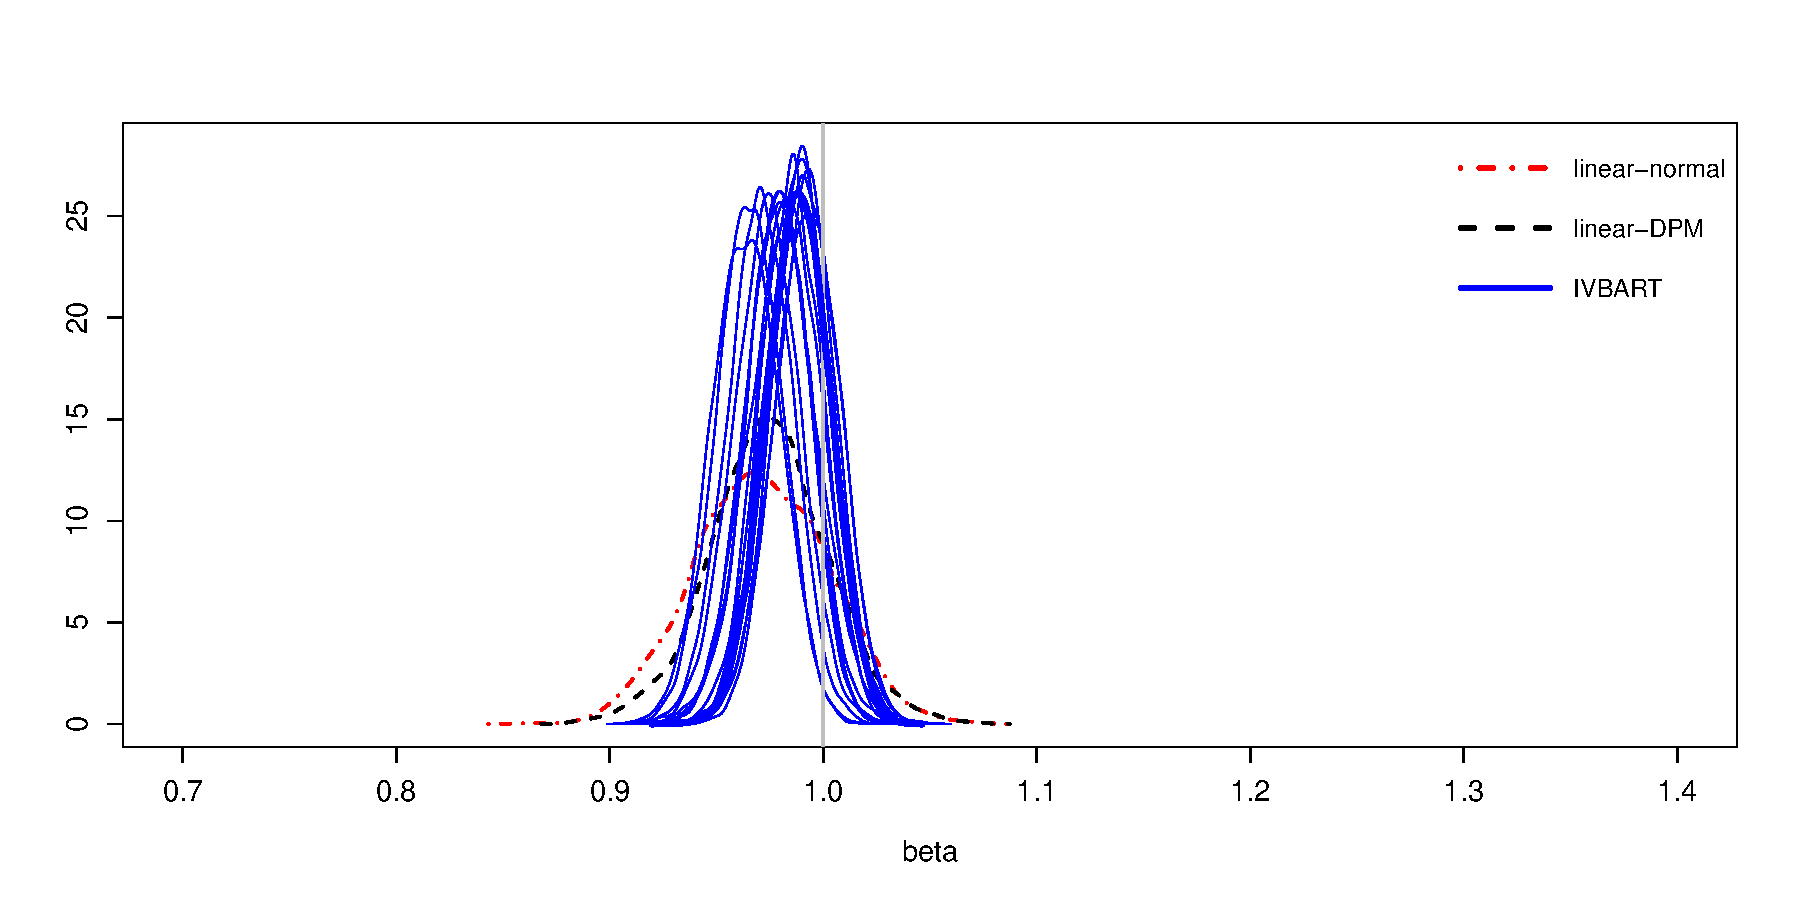
\includegraphics[scale=.6]{14-11_1-2_2000_sim-prisens_2-way.pdf} 
\caption{%
Prior sensitivity with $n = 2,000$.
In the top plot $\sigma_f = \sigma_h$ and these values are varied in $S_\sigma = \{.8,1,1.2,1.4\}$.
In the bottom plot, all 16 density estimates obtained using $\sigma_f \in S_\sigma$ and $\sigma_h \in S_\sigma$
are shown.
The thicker density corresponds to $(\sigma_f,\sigma_h) = (1.2, 1.2)$.
Densities for draws from the linear-normal (dot-dash line) and linear-DPM (dashed line) models are also shown in each plot.
\label{fig:sim-prisens-2000}}
\end{figure}

In practice we view the above sensitivity to be key part of the analysis as in Section~\ref{card} where
we analyze the famous Card data.
We are currenlty researching effective data based default prior choices, but feel than in this model
analysis of prior sensitivity will continue to be an essential part of the investigation.
Note that this is still much simpler than attempting to explore the sensitivity of two-stage least
squares to the inclusion of possible transformed $x$ and $z$.
As currently engineered, our approach is not targeted towards a ``big p'' scenario where we entertain
verly large $x$ or $z$ vectors of variables.
However, we feel the case we have investigated in our simulations with ten $x$ and five $z$ instruments 
is representative of many applied problems.
We explore the ``big p'' problem in future research.

\subsection{Markov Chain Monte Carlo Performance}\label{subsec:sim-mcmc}

In Figure~\ref{fig:mcmc} we take a quick look at the time series characteristics of our
MCMC draws of $\beta$.
Figure~\ref{fig:mcmc} displays time series plots of the $\beta$ draws for a single drawn
sample of $n = 2,000$ observations and the nonlinear choices of $f$ and $h$.

The top left plot displays all draws and the top right displays the corresponding ACF.
The bottom left plot displays draws thinned to keep every tenth and the bottom right displays the corresponding ACF.

While the dependence is strong, we can obtain an effective inference in this case by simply taking
every thenth draw.

\begin{figure}
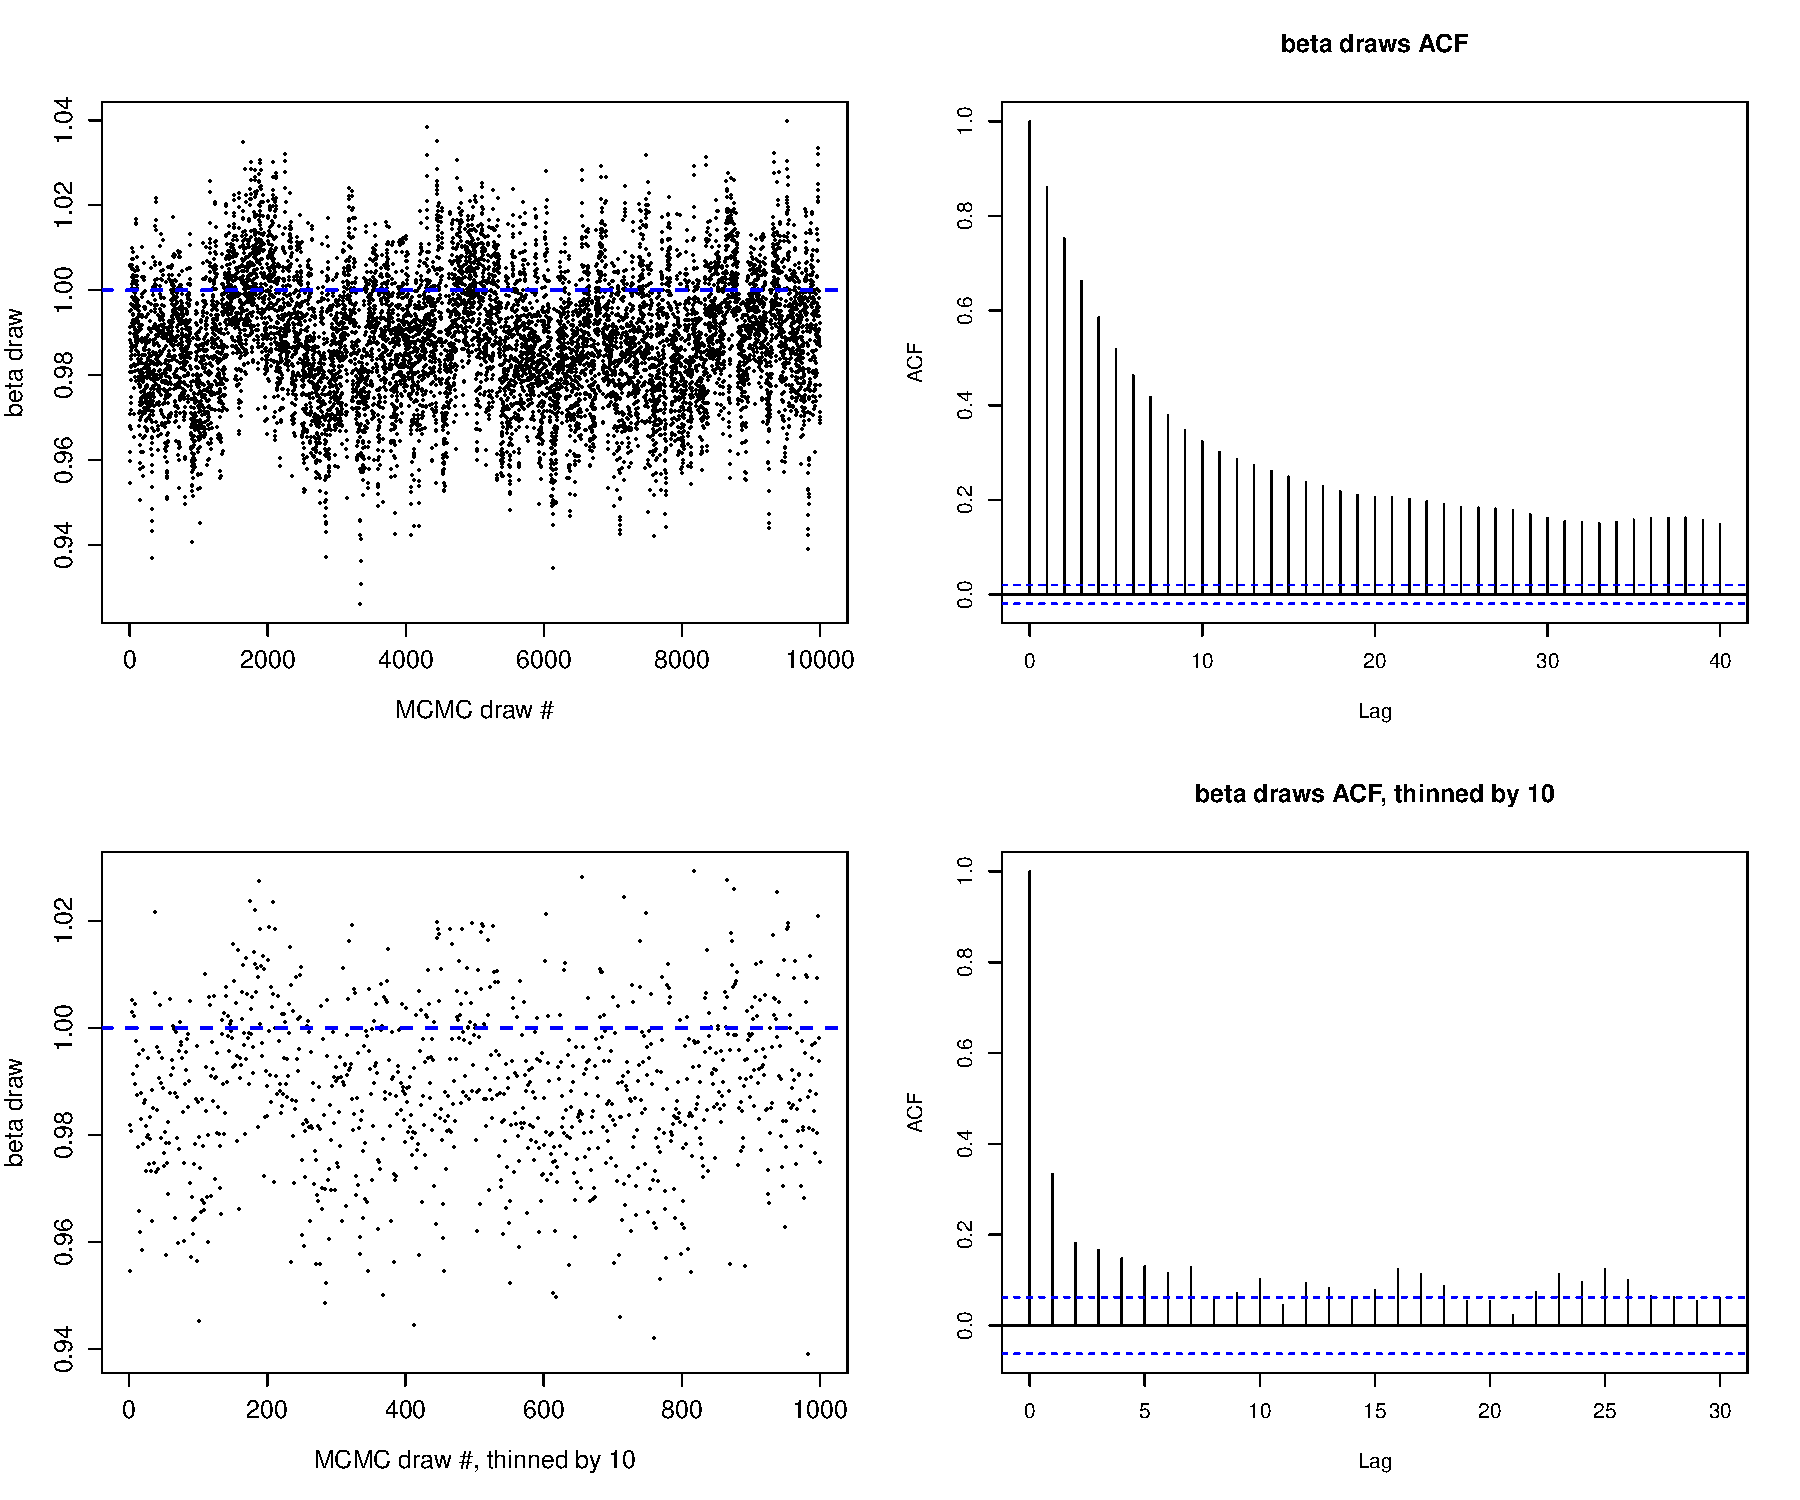
\includegraphics[scale=.6]{14-11_1-2_2000_MCMC.pdf}
\caption{%
Time series behaviour of the $\beta$ MCMC draws.
}\label{fig:mcmc}
\end{figure}
